\subsubsection{Viscosity grooves benchmark}
\label{sec:viscosity_grooves}

\textit{This benchmark was designed by Dave May and this section was contributed by Cedric Thieulot.}

The domain is a two-dimensional Cartesian box of size $L\times L$.
The velocity and pressure fields are given by
\begin{eqnarray}
u(x,y) &=& x^3 y + x^2 + xy + x, \\
v(x,y) &=& -\frac{3}{2}x^2y^2 - 2xy - \frac{1}{2}y^2 - y, \\
p(x,y) &=& x^2y^2 + xy + 5 + p_0,
\end{eqnarray}
where $p_0$ is a constant to be determined based on the type of pressure normalization.
The viscosity is chosen to be
\begin{equation}
\eta(x,y)=-\sin(p)+1+\epsilon = -\sin (x^2y^2 + xy + 5) + 1 + \epsilon,
\end{equation}
where $\epsilon$ controls the viscosity contrast.
It is easy to verify that the flow is incompressible as the velocity field satisfies $\nabla\cdot \mathbf u = 0$.
The right hand side term of the Stokes equation is obtained by inserting
the expressions for velocity, pressure and viscosity in the momentum conservation equation, see \cite{fieldstone} for details.
The velocity, pressure and right hand side magnitude are shown in Figure~\ref{fig:benchmark-grooves-3x3}
for $L=3$ and $\epsilon=0.1$.

The $p_0$ constant can be determined by requiring that the pressure is normalized over the
volume of the domain:
\begin{equation}
\int_\Omega p dV=
\int_0^L\int_0^L p(x,y) \, dx dy =
\int_0^L\int_0^L (x^2y^2+xy+5)\, dx \, dy + \int_0^L \int_0^L p_0 \, dx \, dy =0.
\end{equation}
It then follows that:
\begin{equation}
p_0 =-  \frac{1}{L^2}  \int_0^L\int_0^L (x^2y^2+xy+5) dx dy
= -\frac{L^4}{9}-\frac{L^2}{4} - 5.
\end{equation}

\begin{figure}
\centering
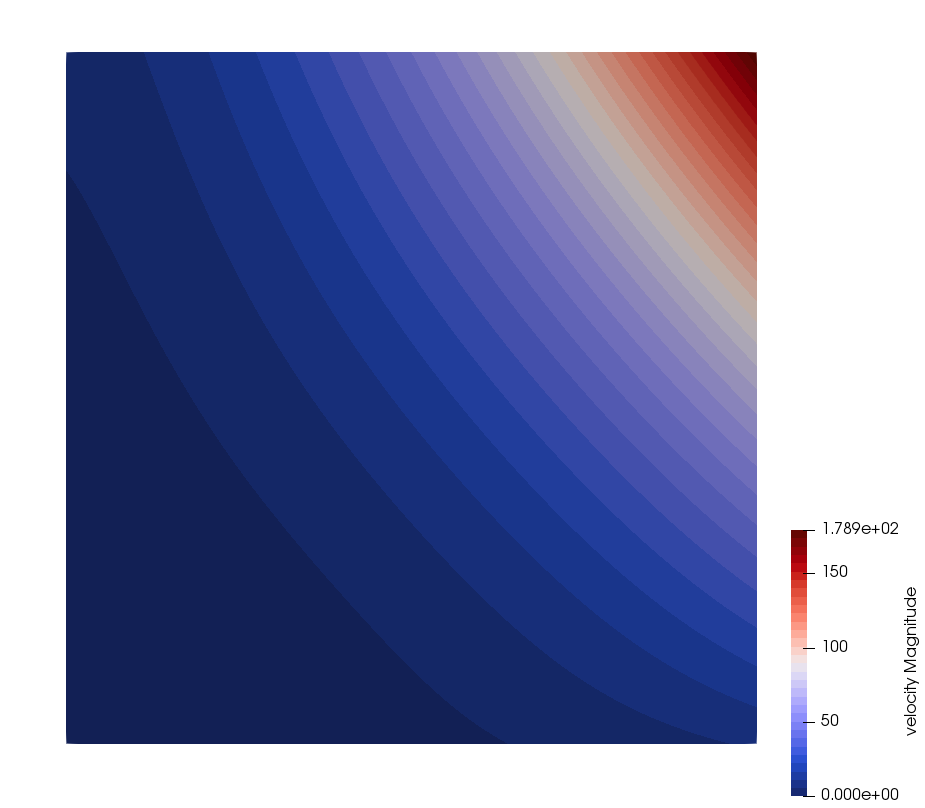
\includegraphics[width=0.31\textwidth]{cookbooks/benchmarks/viscosity_grooves/doc/vel3x3.png}
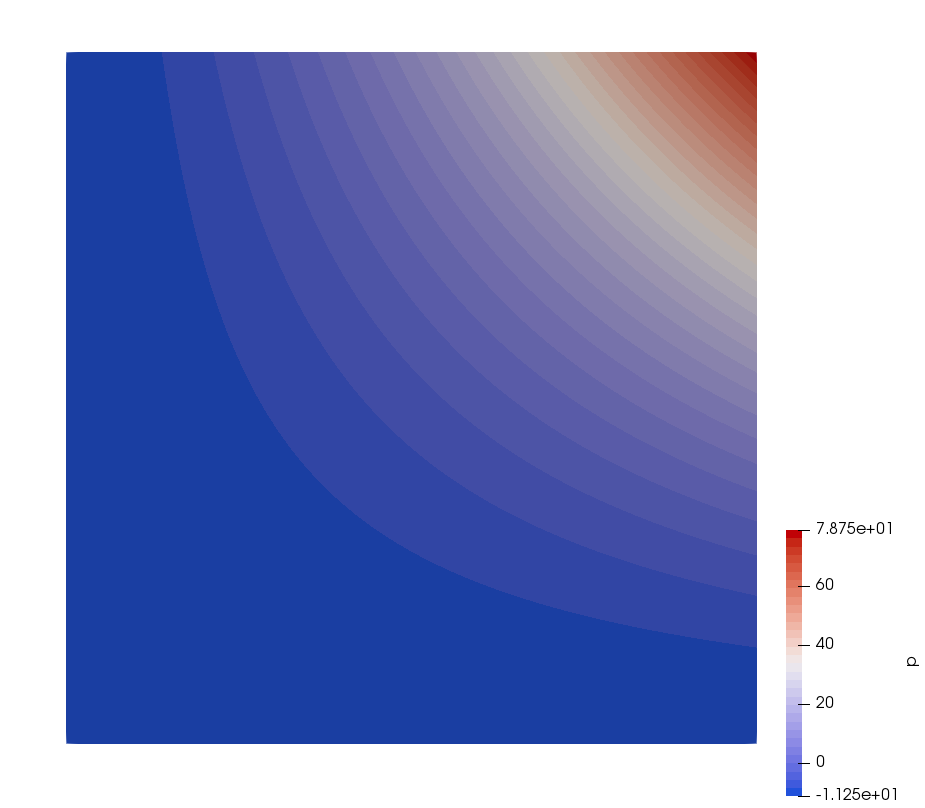
\includegraphics[width=0.31\textwidth]{cookbooks/benchmarks/viscosity_grooves/doc/press3x3.png}
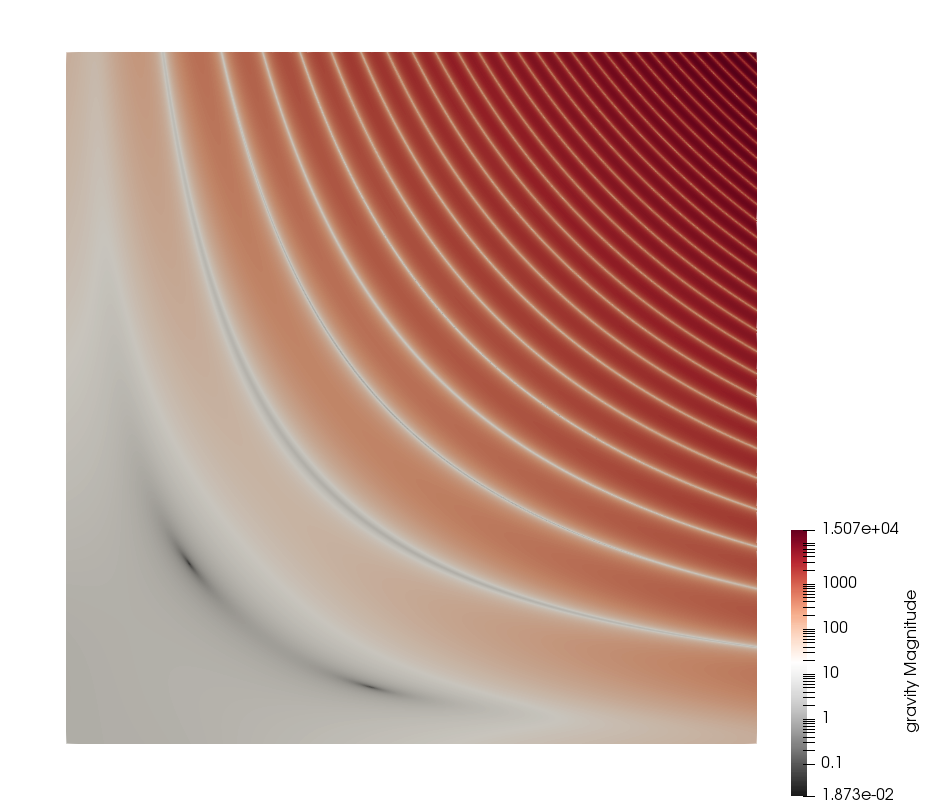
\includegraphics[width=0.31\textwidth]{cookbooks/benchmarks/viscosity_grooves/doc/rhs3x3.png}
\hfill
\caption{\it Viscosity grooves benchmark: From left to right, velocity field, pressure field, and
norm of the right hand side of the momentum equation, for a $3\times 3$ domain
with $\epsilon=0.1$.}
\label{fig:benchmark-grooves-3x3}
\end{figure}

As seen in Figure~\ref{fig:benchmark-grooves-domains}, the value of $\epsilon$ controls the viscosity field amplitude:
when the $\sin$ term of the viscosity takes value 1, the viscosity is then equal to $\epsilon$; when the $\sin$ is
equal to $-1$, the viscosity is then $2+\epsilon$. In other words, the ratio between maximal and minimal
viscosity in the domain is of the order $\frac{2}{\epsilon}$.

Another interesting aspect of this benchmark is the fact that increasing the domain size
adds complexity to it as it increases the number of low viscosity zones and the spacing
between them decreases.

\begin{figure}
\centering
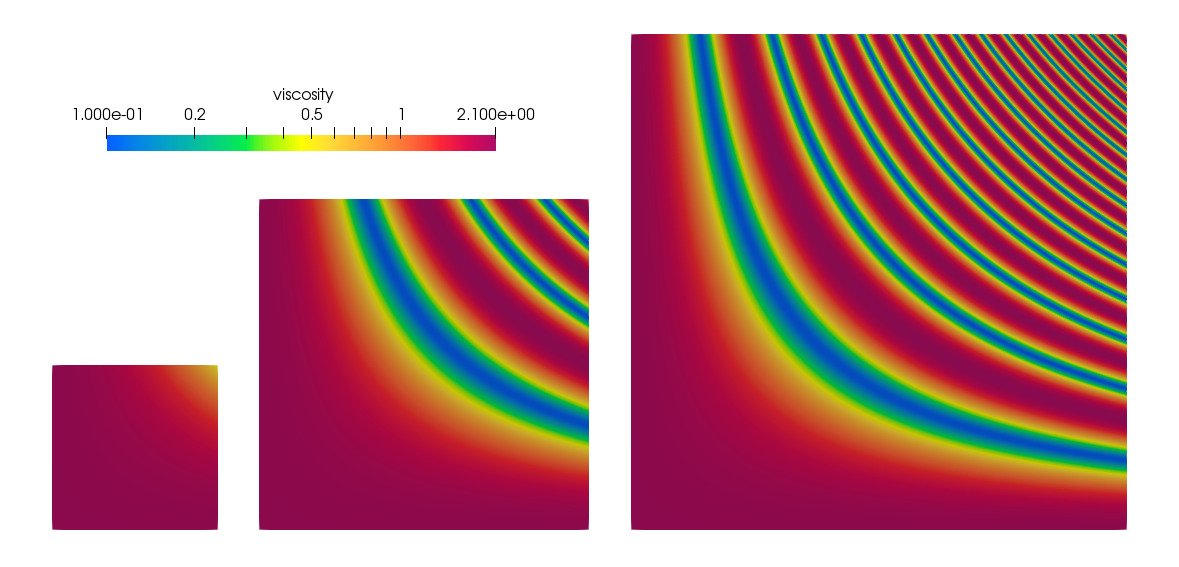
\includegraphics[width=0.9\textwidth]{cookbooks/benchmarks/viscosity_grooves/doc/viscs.png}
\caption{\it Viscosity grooves benchmark: Viscosity field for three domain sizes: $1\times 1$, $2\times 2$ and $3\times 3$.}
\label{fig:benchmark-grooves-domains}
\end{figure}

The velocity and pressure errors (in the $L_2$ norm) are measured for $L=1,2,3$, global refinement
levels 3 to 9 (resolutions $8\times 8$ to $512\times 512$)
and $\epsilon=10^{-1},10^{-2},10^{-3}$. Figure~\ref{fig:benchmark-grooves-errors} shows the velocity and pressure error convergence as a function of the mesh size for $\epsilon=0.1$ (results are identical for the other two $\epsilon$ values).
The expected convergence rates (cubic convergence for velocity and quadratic for pressure) are recovered for the $1\times 1$ domain at all resolutions. These rates are recovered for the $2\times 2$ domain for resolutions above level 6. We find that
the multitude of low viscosity bands in the upper right corner of the $3\times 3$ domain will require a refinement level larger than 9 to recover the optimal convergence rates.

\begin{figure}
\centering
\includesvg[width=0.9\textwidth]{cookbooks/benchmarks/viscosity_grooves/doc/conv_0p1.svg}
\caption{\it Viscosity grooves benchmark: Velocity and pressure error convergence as a function of the mesh size $h$ for 3 domain sizes.}
\label{fig:benchmark-grooves-errors}
\end{figure}
